% $Header: /cvsroot/latex-beamer/latex-beamer/solutions/conference-talks/conference-ornate-20min.en.tex,v 1.7 2007/01/28 20:48:23 tantau Exp $

\documentclass{beamer}

% This file is a solution template for:

% - Talk at a conference/colloquium.
% - Talk length is about 20min.
% - Style is ornate.



% Copyright 2004 by Till Tantau <tantau@users.sourceforge.net>.
%
% In principle, this file can be redistributed and/or modified under
% the terms of the GNU Public License, version 2.
%
% However, this file is supposed to be a template to be modified
% for your own needs. For this reason, if you use this file as a
% template and not specifically distribute it as part of a another
% package/program, I grant the extra permission to freely copy and
% modify this file as you see fit and even to delete this copyright
% notice. 


\mode<presentation>
{
  \usetheme{Dresden}
  % or ...

  \setbeamercovered{transparent}
  % or whatever (possibly just delete it)
}


\usepackage[english]{babel}
% or whatever

\usepackage[latin1]{inputenc}
% or whatever

\usepackage{times}
\usepackage[T1]{fontenc}
% Or whatever. Note that the encoding and the font should match. If T1
% does not look nice, try deleting the line with the fontenc.


\title[D-Wave] % (optional, use only with long paper titles)
{Adiabatic Quantum Computation}

\subtitle
{at D-Wave Systems Inc.}

\author[Carson Holgate] % (optional, use only with lots of authors)
{Carson~Holgate}
% - Give the names in the same order as the appear in the paper.
% - Use the \inst{?} command only if the authors have different
%   affiliation.

\institute[NCSU] % (optional, but mostly needed)
{
  \inst{}
  Computer Science\\
  Math\\
  NCSU
}
% - Use the \inst command only if there are several affiliations.
% - Keep it simple, no one is interested in your street address.

\date[MA591 2010] % (optional, should be abbreviation of conference name)
{MA 591 Special Topics in Quantum Computation}
% - Either use conference name or its abbreviation.
% - Not really informative to the audience, more for people (including
%   yourself) who are reading the slides online

\subject{Physical Realizations of Quantum Computation}
% This is only inserted into the PDF information catalog. Can be left
% out. 



% If you have a file called "university-logo-filename.xxx", where xxx
% is a graphic format that can be processed by latex or pdflatex,
% resp., then you can add a logo as follows:

% \pgfdeclareimage[height=0.5cm]{university-logo}{university-logo-filename}
% \logo{\pgfuseimage{university-logo}}



% Delete this, if you do not want the table of contents to pop up at
% the beginning of each subsection:
\AtBeginSubsection[]
{
  \begin{frame}<beamer>{Outline}
    \tableofcontents[currentsection,currentsubsection]
  \end{frame}
}


% If you wish to uncover everything in a step-wise fashion, uncomment
% the following command: 

%\beamerdefaultoverlayspecification{<+->}


\begin{document}

\begin{frame}
  \titlepage
\end{frame}

\begin{frame}{Outline}
  \tableofcontents
  % You might wish to add the option [pausesections]
\end{frame}


% Structuring a talk is a difficult task and the following structure
% may not be suitable. Here are some rules that apply for this
% solution: 

% - Exactly two or three sections (other than the summary).
% - At *most* three subsections per section.
% - Talk about 30s to 2min per frame. So there should be between about
%   15 and 30 frames, all told.

% - A conference audience is likely to know very little of what you
%   are going to talk about. So *simplify*!
% - In a 20min talk, getting the main ideas across is hard
%   enough. Leave out details, even if it means being less precise than
%   you think necessary.
% - If you omit details that are vital to the proof/implementation,
%   just say so once. Everybody will be happy with that.

\section{Adiabatic Quantum Computation}

\subsection{Adiabatic Theorem}

\begin{frame}{Adiabatic Theorem}{Max Born and Vladimir Fock (1928)}
  % - A title should summarize the slide in an understandable fashion
  %   for anyone how does not follow everything on the slide itself.
  \texttt{A physical system remains in its instantaneous eigenstate if a given perturbation is acting on it slowly enough and if there is a gap between the eigenvalue and the rest of the Hamiltonian's spectrum.}
  
\end{frame}

\subsection{Application of Adiabatic Theorem}

\begin{frame}{Application}

  \begin{itemize}
    \item Quantum systems evolve according to the Schr\"{o}dinger equation.
     \[ i \frac{d}{dt} |\psi(t)\rangle = \mathcal{H}(t)|\psi(t)\rangle\]
    \pause
   \item Start with \(|\psi(0)\rangle\) as the ground state of \(\mathcal{H}(0)\).
    \pause
   \item If there is a non-zero gap between \(|\psi(0)\rangle\), and the next lowest energy level as long as \(\mathcal{H}(t)\) varies slowly enough (i.e. little energy is added to the system) \(|\psi(t)\rangle\) will remain close to the instantaneous ground state of \(\mathcal{H}(t)\).
  \end{itemize}

\end{frame}

\begin{frame}{The Magic}
\pause
  \begin{itemize}
   \item Encode the solution in the ground state of a problem Hamiltonian \(\mathcal{H}_P\).
    \begin{itemize}
     \item Specifying \(\mathcal{H}_P\) is easy but finding its ground state is difficult.
    \end{itemize}
    \pause
   \item Choose an initial Hamiltonian \(\mathcal{H}_B\) whose ground state is easy to find.
    \pause
   \item Construct the system: \[\mathcal{H}(t) = (1-t/T)\mathcal{H}_B + (t/T)\mathcal{H}_P\] Where T is a parameter to control the rate at which \(\mathcal{H}(t)\) varies.  Normalized to \(\tilde{\mathcal{H}}(s), 0 \leq s\leq 1\): \[\tilde{\mathcal{H}}(s) = (1-s)\mathcal{H}_B + s\mathcal{H}_P\]

  \end{itemize}

\end{frame}

\section{D-Wave}

\subsection{Background}

\begin{frame}{History}
 \begin{itemize}
  \item Founded in 1999 by:
    \begin{itemize}
     \item Haig Farris
     \item Geordie Rose (CTO)
     \item Bob Wiens (former CFO)
     \item Alexandre Zagoskin (Chief Scientist)
    \end{itemize}
   \item Started as an off-shoot of the University of British Columbia funding academic research in quantum computing.
   \item Currently located in Burnaby, British Columbia.

 \end{itemize}

\end{frame}

\begin{frame}{Goals}
 
 \begin{itemize}
  \item Find low cost solutions to Quadratic Unconstrained Binary Optimization (QUBO) problems.
  \begin{itemize}
   \item arXiv:quant-ph/0001106v1 3-SAT
   \item NPC controversy
  \end{itemize}
  \pause
  \item Equivalent to finding low energy states of classical Ising Hamiltonian: \[\mathcal{H} = \displaystyle\sum\limits_{i}h_i\sigma_{zi} + \displaystyle\sum\limits_{ij}J_{ij}\sigma_{zi}\sigma_{zj}\]
  \pause
  \item Find a reasonable way to do it
 \end{itemize}

\end{frame}

\subsection{Chimera C4 Chip}

\begin{frame}{Infrastructure}

  \begin{center}
 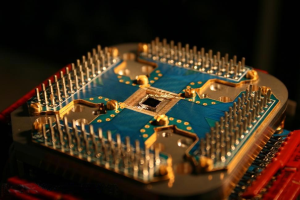
\includegraphics[scale=.2]{../img/13073_D_Wave_Orion_16_Qubit}
 \end{center}
 
 \begin{itemize}
  \item Superconducting metals operating at ultra low temperatures
  \item Manufactured with existing fabrication techniques
 \end{itemize}

\end{frame}

\begin{frame}{The Qubit}
 \begin{center}
  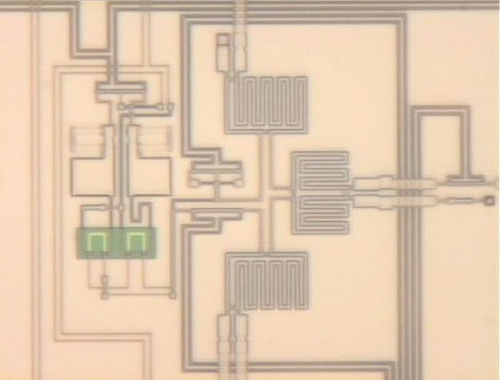
\includegraphics[scale=.7]{../img/Real_Qubit}
 \end{center}

\end{frame}

\begin{frame}{Schematic}
 \begin{center}
  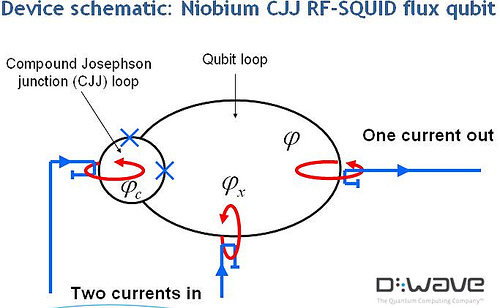
\includegraphics[scale=.7]{../img/Qubit_Schematic}
 \end{center}

\end{frame}

\begin{frame}{System}
 \begin{center}
  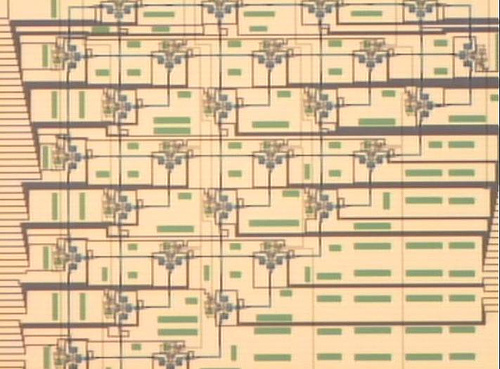
\includegraphics[scale=.7]{../img/Qubit_System}
 \end{center}

\end{frame}

\subsection{Applications}

\begin{frame}{Orion}
\begin{center}
 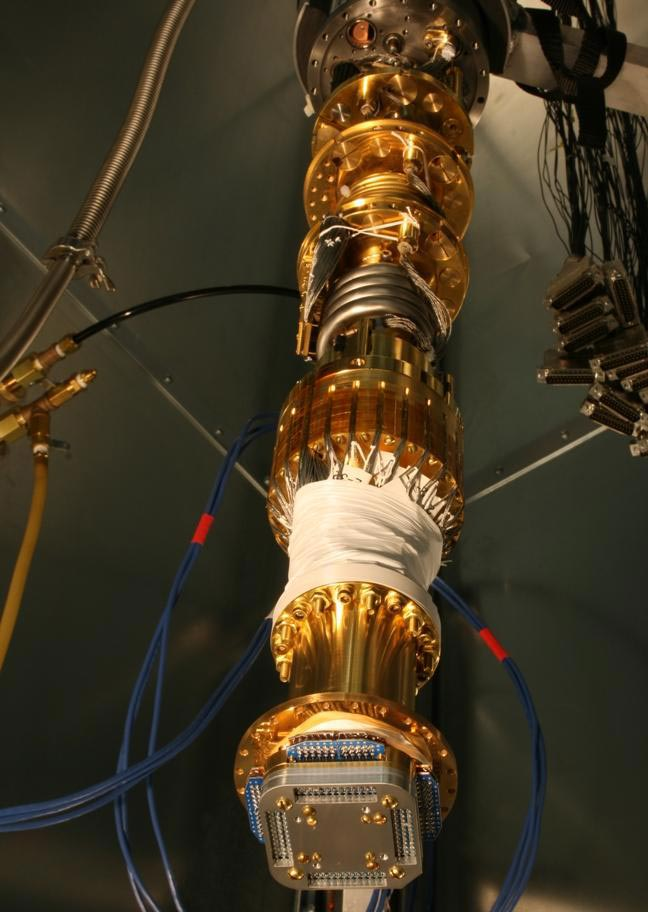
\includegraphics[scale=.125]{../img/Orion}
  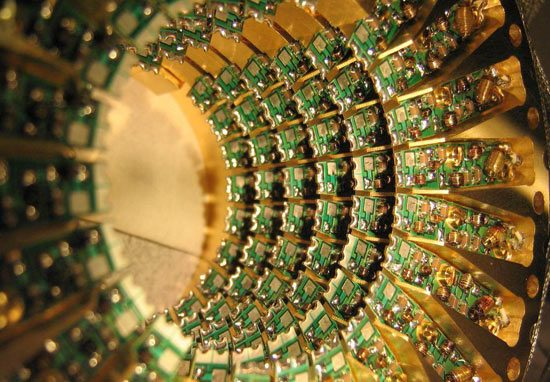
\includegraphics[scale=.3]{../img/Open_Orion}
\end{center}
 
\begin{itemize}
  \item 16 qubit System
  \begin{itemize}
   \item www.apps.dwavesys.com
   \item Orion web services API
  \end{itemize}

 \end{itemize}

\end{frame}

\begin{frame}{Google's Interest}
 \begin{itemize}
  \item Image matching
  \begin{itemize}
   \item Google Goggles
   \item Face Recognition
  \end{itemize}
  \item Machine learning
  \begin{itemize}
   \item Recognizing cars
  \end{itemize}

 \end{itemize}

\end{frame}

\section{Controversy}

\subsection{Is it Really a Quantum Computer?}

\begin{frame}{DiVincenzo}
 \begin{enumerate}
  \item A scalable physical system with well characterized qubits
  \pause
  \item The ability to initialize state
  \pause
  \item Long relevant decoherence times
  \pause
  \item Universal set of quantum gates
  \pause
  \item The ability to measure specific quibits
 \end{enumerate}

\end{frame}

\subsection{Complexity Theory}

\begin{frame}{P == NP?}
 \begin{itemize}
  \item QUBO \(\supset\) P
  \pause
  \item Goldstone, Gutmann, and Sipser adiabatic algorithmic solution for 3-SAT
  \item Aharonov, van Dam, et al adiabatic quantum computation is equivalent to standard computation (NMR)
  \pause
  \item Problems with simulated annealing
  \begin{itemize}
   \item QUBO solutions are only NP-Hard
  \end{itemize}


 \end{itemize}

\end{frame}


\section*{Summary}

\begin{frame}{Summary}

  % Keep the summary *very short*.
  \begin{itemize}
  \item
    Adiabatic quantum computating is feasible with current manufacturing techniques and because of long decoherence times.
  \item
    The Chimera C4 chip has been demonstrated successfully.
  \item
    The actual quantum nature of the system is controversial.
  \end{itemize}
  
  % The following outlook is optional.
  \vskip0pt plus.5fill
  \begin{itemize}
  \item
    Outlook
    \begin{itemize}
    \item
      D-Wave has yet to produce a fully entangled system due to bus connectivity issues.
    \item
      The backend of Orion is still a simulation but should be up and running soon.
    \end{itemize}
  \end{itemize}
\end{frame}



% All of the following is optional and typically not needed. 
\appendix
\section<presentation>*{\appendixname}
\subsection<presentation>*{More Resources}

\begin{frame}[allowframebreaks]
  \frametitle<presentation>{More Resources}
    
  \begin{thebibliography}{10}
 
    
  \beamertemplatearticlebibitems
  % Followed by interesting articles. Keep the list short. 
  \bibitem{AQC=SQC2005}
    D.~Aharonov, W.~vanDam, J.~Kempe, Z.~Landau, S.~Lloyd, O.~Regev
    \newblock Adiabatic Quantum Computation is Equivalent to Standard Quantum Computation.
    \newblock {\em arXiv:quant-ph/0405098v2},2005.
  
  \bibitem{PIQC2000}
    D.~DiVincenzo.
    \newblock The Physical Implementation of Quantum Computation.
    \newblock {\em arXiv:quant-ph/0002077v3},2000.

  \bibitem{AQC2000}
    E.~Farhi, J.~Goldstone, S.~Gutmann, M.~Sipser
    \newblock Quantum Computation by Adiabatic Evolution.
    \newblock {\em arXiv:quant-ph/0001106v1},2000.

  \bibitem{RSFQ2009}
    R.~Harris et al.
    \newblock Experimental Demonstration of a Robust and Scalable Flux Qubit
    \newblock {\em arXiv:0909.4321v1 [cond-mat.supr-con]},2009.

  \bibitem{GRB2009}
    H.~Neven
    \newblock Machine Learning with Quantum Algorithms
    \newblock {\em http://googleresearch.blogspot.com/2009/12/machine-learning-with-quantum.html},2009.

  \bibitem{GRBlog2010}
    G.~Rose
    \newblock rose.blog
    \newblock {\em http://dwave.wordpress.com/}

  \bibitem{GTT2007}
    H.~Neven, G.~Rose
    \newblock Google Tech Talks: Quantum Computing
    \newblock {\em http://www.youtube.com/watch?v=I56UugZ_8DI&feature=channel},2007.

  \bibitem{dwavesite2010}
    \newblock D-Wave Systems Inc.
    \newblock {\em http://www.dwavesys.com/}

  \end{thebibliography}
\end{frame}

\end{document}


